%%%%%%%%%%%%%%%%%%%%%%%%%%%%%%%%%%%%%%%%%%%%%%%%%%%%%%%%%%%%%%%%%%%%%%%%%%%%%%%%%%%%%%%%%
% This is a LaTeX template for Bachelor or Master theses at ZHAW, in accordance with the 
% guidelines provided here:
% https://www.zhaw.ch/en/lsfm/study/studiweb/master-ls/masters-thesis/
%
%
% This template is based on previous works by:
% Steve Gunn (http://users.ecs.soton.ac.uk/srg/softwaretools/document/templates/)
% Sunil Patel (http://www.sunilpatel.co.uk/thesis-template/)
% Matteo Delucchi (https://github.com/matteodelucchi/ZHAW_thesis-template)
%
% University specific changes were made by:
% Matteo Delucchi
% Norman Juchler
% 
% Template license:
% CC BY-NC-SA 3.0 (http://creativecommons.org/licenses/by-nc-sa/3.0/)
%%%%%%%%%%%%%%%%%%%%%%%%%%%%%%%%%%%%%%%%%%%%%%%%%%%%%%%%%%%%%%%%%%%%%%%%%%%%%%%%%%%%%%%%%

%----------------------------------------------------------------------------------------
% DOCUMENT SPECIFICATION
%----------------------------------------------------------------------------------------
\documentclass[
    11pt,                      % Default font size
    %oneside,                  % One-side binding. Default: Two-side binding / alternating margins
    english,                   % Language. Use ngerman for German (Neue Rechtschreibung)
    singlespacing,             % Spacing option: singlespacing, onehalfspacing or doublespacing
    %nolistspacing,            % Set spacing in lists to single
    %draft,                    % Enable draft mode: no pictures, no links, overfull hboxes indicated
    liststotoc,               % Include list of figures/tables/etc in the table of contents
    %toctotoc,                 % Include the main table of contents to the table of contents
    parskip,                  % Add vertical space between paragraphs
    %nohyperref,               % Disable links in the entire document
    headsepline,               % Show a horizontal line under the header
    %chapterinoneline,         % Place the chapter title and chapter number on one line
    consistentlayout,          % Have the same layout for special chapters: 
                               % declaration, abstract and acknowledgements
]{MastersDoctoralThesis}

% Uncomment the following lines to only include a subset of chapters.
% This is useful for long documents, as typesetting takes a bit of time
%\includeonly{
%    front/titlepage,
%    front/imprint,
%    front/abstract,
%    %front/declaration,
%    %front/acknowledgements,
%    %front/symbols,
%    Chapters/Chapter1,
%    %Chapters/Chapter2
%    }


%----------------------------------------------------------------------------------------
% PREAMBLE: PACKAGES AND CONFIGURATIONS
%----------------------------------------------------------------------------------------
% !TEX root = main.tex

%----------------------------
%   Fonts and characters
%----------------------------

% Support for special characters
\usepackage[utf8]{inputenc}    % Specify input encoding
\usepackage[T1]{fontenc}       % Specify font encoding

% Set main fonts
% Fonts catalogue: https://tug.org/FontCatalogue/
\usepackage{mathpazo}          % Use the Palatino font by default
\usepackage{beramono}          % Override the monospace/typewriter font

% ZHAW title font
% Try to load Helvetica Rounded Bold, and OpenType font.
% Loading OTF or system fonts is possible with XeLaTeX.
% If the document is compiled using pdfLaTeX, resort 
\usepackage{ifxetex}
\ifxetex
    \usepackage{fontspec}
    \newfontfamily\zhawtitlefont{Helvetica Rounded Bold}
\else
    \newcommand{\zhawtitlefont}{\scshape}
\fi

%\usepackage[scaled]{helvet}

%----------------------------
%   Environments
%----------------------------

\usepackage{caption}           % Customized caption
\usepackage{subcaption}        % Subfigure captions
\usepackage{makecell}          % Per-cell formatting in tables (\makecell)
\usepackage{pdfpages}          % Required to include PDF files/graphics (\includepdf)
\usepackage{outlines}
\usepackage{url}

\usepackage{todonotes}         % Introduces the command \todo
\setlength{\marginparwidth}{2.5cm} % Adjust this if the todo notes are out of margins

% Create boxes as follows:
% \begin{colorbox}{red}{2}
\usepackage{tcolorbox}
\newtcolorbox{textbox}[2]{
    arc=3pt,
    boxrule=#2pt,
    colback=#1!25!white,
    width=\textwidth,
    halign=left,
    valign=center,
    colframe=#1!75!black
}

%----------------------------
%   Colors
%----------------------------

% Set up colors
\usepackage{xcolor}
% ZHAW Blue: Pantone 2945 U / R0 G100 B166
\definecolor{zhawblue}{rgb}{0.00, 0.39, 0.65}
% Colors related to code listings
\definecolor{codegreen}{rgb}{0,0.6,0}
\definecolor{codegray}{rgb}{0.5,0.5,0.5}
\definecolor{codepurple}{rgb}{0.58,0,0.82}
\definecolor{codebackground}{rgb}{0.93,0.94,0.95}

%----------------------------
%   Code listings
%----------------------------

% Setup code listings
\usepackage{listings}
\lstdefinestyle{mystyle}{
    backgroundcolor=\color{codebackground},   
    commentstyle=\color{codegreen},
    keywordstyle=\color{magenta},
    numberstyle=\tiny\color{codegray},
    stringstyle=\color{codepurple},
    basicstyle=\ttfamily\footnotesize,
    breakatwhitespace=false,
    breaklines=true,
%    captionpos=b,
    keepspaces=true,
    numbers=left,
    numbersep=5pt,
    showspaces=false,
    showstringspaces=false,
    showtabs=false,
    tabsize=4
}
\lstset{style=mystyle}

% minted is an alternative code listing package. (See chapter 2)
% For it to run successfully, ensure the following:
% - the Python package Pygments. Install with the following command:
%       python -m pip install Pygments
% - pdflatex (or xelatex) is executed with the flag --shell-escape
%   If you are using a TEX editor, you can modify the typesetting 
%   command somewhere in the settings.
%\usepackage[outputdir=build]{minted}
%\usemintedstyle{xcode}
% For fancier coloring schemes, see here:
% https://tex.stackexchange.com/questions/585582
% One could also create an own style in Pygments
% https://pygments.org/docs/styles/#creating-own-styles

%----------------------------
%   References
%----------------------------

% Set up references
\usepackage[
    backend=biber,             % Use biber backend (an external tool)
    sorting=none,              % Enumerates the reference in order of their appearance
    style=numeric-comp         % Choose here your preferred citation style
]{biblatex}
\addbibresource{example.bib}   % The filename of the bibliography
\usepackage[autostyle=true]{csquotes} 
                               % Required to generate language-dependent quotes 
                               % in the bibliography

%----------------------------------------------------------------------------------------
%   MARGIN SETTINGS
%----------------------------------------------------------------------------------------

\geometry{
    paper=a4paper,      % Change to letterpaper for US letter
    inner=2.5cm,        % Inner margin
    outer=3.8cm,        % Outer margin
    top=1.5cm,          % Top margin
    bottom=1.5cm,       % Bottom margin
    bindingoffset=.5cm, % Binding offset
    %showframe,         % Show the type block of the page
}
\setlength{\parskip}{1em}
\usepackage{enumitem}          % Layout control for list environments (e.g, itemize)
%\setlist{noitemsep}           % Suppress extra spaces between items
%\setlist{nosep}               % Suppress spaces before/after list environments

\usepackage{graphicx}
\usepackage{float}
\tcbuselibrary{skins, raster}
\usepackage{acronym}

\usepackage{glossaries}

\makeglossaries


%----------------------------------------------------------------------------------------
% THESIS INFORMATION: MODIFY THIS SECTION!
%----------------------------------------------------------------------------------------

% The information below is used in the following parts:
% - Title page
% - Imprint
% - Abstract / Zusammenfassung
% - Meta information of PDF

\thesistitle{Project Title}             % Thesis title,              command: \ttitle
\thesistype{Track Module 1}             % Type of thesis (e.g. Master Thesis) \ttype
\thesisdate{\today}                     % Date of submission                  \tdate
\keywords{gravity, physics, disruptive science}
                                        % Keywords for the thesis,            \keywordnames
\author{Maxine Muster}                  % Your name,                          \authorname
\degree{Master of Science ZFH}          % Degree name,                        \degreename
\studyprogram{Applied Computational Life Sciences, M.Sc.} 
                                        % Study program                       \studyprog
\studyprogramlink{https://www.zhaw.ch/en/lsfm/study/master/applied-computational-life-sciences/}
                                        % Link to study program               \studyproglink

\supervisorA{Dr. Albert Einstein}       % Name of supervisor 1,               \supnameA
\supervisorAmail{e=mc2@zhaw.ch}         % Email address of supervisor 1,      \supmailA
\supervisorAweb{https://en.wikipedia.org/wiki/Albert\_Einstein}  %            \supwebA
\supervisorAinfo{                       % Formatted info about supervisor 1:  \supinfoA
    \supnameA\\
    Zurich University of Applied Sciences\\
    Email: \href{mailto:\supmailA}{\supmailA}\\
    Web: \href{\supwebA}{Link}
}

% Keep empty if there is no supervisor 2: \supervisorB{}
\supervisorB{Isaac Newton}              % Name of supervisor 2,               \supnameB
\supervisorBmail{f=am@newton.com}       % Email address of supervisor 2,      \supmailB
\supervisorBweb{https://en.wikipedia.org/wiki/John\_Locke}                  % \supwebB
\supervisorBinfo{                       % Formatted info about supervisor 2:  \supinfoB
    \supnameB\\
    University of Cambridge\\
    Email: \href{mailto:\supmailB}{\supmailB}\\
    Web: \href{\supwebB}{Link}
}

\university{Zurich University of Applied Sciences}
                                        % University name                     \univname
\universitygerman{Zürcher Hochschule für Angewandte Wissenschaften}
                                        % University, in German               \univnameger
\department{Life Sciences and Facility Management} 
                                        % Department,                         \deptname
\institute{Institute of Computational Life Sciences} 
                                        % Institute,                          \instname
\group{Center of Computational Health} 
                                        % Research group                      \groupname

% Links
\universitylink      {https://www.zhaw.ch/en/university/}                   % \univlink
\universitylinkgerman{https://www.zhaw.ch/de/university/}                   % \univlinkger
\departmentlink      {https://www.zhaw.ch/de/lsfm/}                         % \deptlink
\institutelink       {https://www.zhaw.ch/en/lsfm/institutes-centres/icls/} % \instlink
\grouplink           {https://www.zhaw.ch/en/lsfm/institutes-centres/icls/computational-health/} % \grplink



\AtBeginDocument{
\hypersetup{pdftitle=\ttitle} % Set the PDF's title to your title
\hypersetup{pdfauthor=\authorname} % Set the PDF's author to your name
\hypersetup{pdfkeywords=\keywordnames} % Set the PDF's keywords to your keywords
}

\begin{document}
\frontmatter                  % Roman page numbering for the pre-content pages
\pagestyle{plain}             % Default to the plain heading style until the thesis style 
                              % is called for the body content


%----------------------------------------------------------------------------------------
% TITLE PAGE AND IMPRINT
%----------------------------------------------------------------------------------------
% !TEX root = ../main.tex

%----------------------------------------------------------------------------------------
% TITLE PAGE
%----------------------------------------------------------------------------------------

\newgeometry{margin=1in}
\begin{titlepage}

% Make the title page mostly inert to the parskip-setting.
\setlength{\parskip}{0pt}

\begin{center}

\includegraphics[width=0.15\textwidth]{Figures/zhaw_rgb}

\ifxetex
    \vspace{0.6cm}
    {\zhawtitlefont\color{zhawblue}\LARGE \univname\par}   % University
    \vspace{0.2cm}
\else
    \vspace{0.87cm}
    {
\includegraphics[height=17.9pt]{Figures/zhaw_font_eng_font}\par}
    \vspace{0.05cm}
\fi
{\Large Department \deptname\par}                      % Department
\vspace{0.2cm}
\vspace{3.5cm}                            
\textsc{\Large \ttype}                                 % Thesis type
\vspace{0.2cm}
\HRule 
\vspace{0.4cm}
{\huge \bfseries \ttitle\par}                          % Thesis title
\vspace{0.4cm}  
\HRule
\vspace{1.5cm}

 
\begin{minipage}[t]{0.4\textwidth}
\begin{flushleft} 
    \large
    \emph{Author:}\\
    \authorname
\end{flushleft}
\end{minipage}
\begin{minipage}[t]{0.4\textwidth}
\begin{flushright} 
    \large
    \emph{Supervisors:} \\
    \supnameA 
\end{flushright}
\end{minipage}
\vspace{2cm}
 
\vfill

{\large
Submitted on\\
\tdate\\
\vspace{1.5cm}
}
\vfill
\end{center}
\end{titlepage}
\restoregeometry

\let\cleardoublepage\clearpage
% !TEX root = ../main.tex

%----------------------------------------------------------------------------------------
% IMPRINT
%----------------------------------------------------------------------------------------

\thispagestyle{empty}
\vspace*{\fill}

{\bfseries  \Large Imprint}
\vspace{0.75cm}

\begin{footnotesize}


\begin{flushleft} 
\begin{tabular}{ @{}lp{0.6\textwidth}@{} } 
\emph{Project:}  & \ttype\\ 
\emph{Title}:    & \ttitle\\
\emph{Author}:   & \authorname\\
\emph{Date}:     & \tdate\\
\emph{Keywords}: & \keywordnames\\
\emph{Copyright}:& \univname

\end{tabular}
\end{flushleft}

\vspace{0.75cm}


\begin{minipage}[t]{0.95\textwidth}
\begin{flushleft} 
\emph{Study program:}\\
\href{\studyproglink}{\studyprog}\\
\href{\univlink}{\univname}
\end{flushleft}
\end{minipage}

\vspace{0.75cm}

\begin{minipage}[t]{0.50\textwidth}
\begin{flushleft} 
\emph{Supervisor 1:}\\
\supinfoA
\end{flushleft}
\end{minipage}
\begin{minipage}[t]{0.45\textwidth}
\begin{flushleft} 
\ifdefempty{\supnameB}
{}
{
    \emph{Supervisor 2:}\\
    \supinfoB
}
\end{flushleft}
\end{minipage}

\end{footnotesize}



%----------------------------------------------------------------------------------------
% DECLARATION
%----------------------------------------------------------------------------------------
% Comment out this section if the declaration of originality from ZHAW is used.
% !TEX root = ../main.tex

%----------------------------------------------------------------------------------------
% DECLARATION OF ORIGINALITY
%----------------------------------------------------------------------------------------

\begin{declaration}
\addchaptertocentry{\authorshipname} % Add the declaration to the table of contents

\begin{textbox}{red}{2}
REMOVE THIS SECTION IF THE \href{https://www.zhaw.ch/en/lsfm/study/studiweb/master-ls/masters-thesis/}{ORIGINAL COPY OF THE ZHAW DECLARATION OF ORIGINALITY} IS USED IN THE APPENDIX.
\end{textbox}
\vspace{1cm}

\noindent I, \authorname, declare that this thesis titled, \enquote{\ttitle} and the work presented in it are my own. I confirm that:

\begin{itemize} 
\item This work was done wholly or mainly while in candidature for a research degree at the \univname.
\item Where any part of this thesis has previously been submitted for a degree or any other qualification at this university or any other institution, this has been clearly stated.
\item Where I have consulted the published work of others, this is always clearly attributed.
\item Where I have quoted from the work of others, the source is always given. With the exception of such quotations, this thesis is entirely my own work.
\item I have acknowledged all main sources of help.
\item Where the thesis is based on work done by myself jointly with others, I have made clear exactly what was done by others and what I have contributed myself.\\
\end{itemize}
\vspace{1cm}

\noindent Signed:\\
\rule[0.5em]{25em}{0.5pt} % This prints a line for the signature
 
\noindent Date:\\
\rule[0.5em]{25em}{0.5pt} % This prints a line to write the date
\end{declaration}

\cleardoublepage


%----------------------------------------------------------------------------------------
% ABSTRACT
%----------------------------------------------------------------------------------------
% !TEX root = ../main.tex

%----------------------------------------------------------------------------------------
% ABSTRACT PAGE
%----------------------------------------------------------------------------------------
\begin{abstract}
\addchaptertocentry{\abstractname} % Add the abstract to the table of contents
The abstract is like a miniature version of the entire manuscript. Structure it similarly: Begin with the context and motivation for the project, a brief description of the method and available data, your findings, and conclusions. Limit yourself to one page!
\end{abstract}


%----------------------------------------------------------------------------------------
% German ABSTRACT PAGE
%----------------------------------------------------------------------------------------
\begin{extraAbstract}
\addchaptertocentry{\extraabstractname} % Add the abstract to the table of contents

Die Zusammenfassung entspricht einer Miniaturversion des gesamten Dokuments. Gliedere sie ähnlich: Beginne mit dem Kontext und der Motivation für das Projekt, einer kurzen Beschreibung der Methode und der verfügbaren Daten, Ihren Ergebnissen und den Schlussfolgerungen. Beschränke dich auf eine Seite!    
\end{extraAbstract}



%----------------------------------------------------------------------------------------
% ACKNOWLEDGEMENTS
%----------------------------------------------------------------------------------------
% !TEX root = ../main.tex

%----------------------------------------------------------------------------------------
% ACKNOWLEDGEMENTS
%----------------------------------------------------------------------------------------
\begin{acknowledgements}
\addchaptertocentry{\acknowledgementname} % Add the acknowledgements to the table of contents

The acknowledgements belong here. Do not forget to mention your project supervisors, without flattering them too much.
\end{acknowledgements}



%----------------------------------------------------------------------------------------
% LIST OF CONTENTS/FIGURES/TABLES PAGES
%----------------------------------------------------------------------------------------
% Comment out if any of the following is not needed:
\tableofcontents  % Add main table of contents
%\listoffigures    % Add list of figures
%\listoftables     % Add list of tables


%----------------------------------------------------------------------------------------
% ABBREVIATIONS / SYMBOLS
%----------------------------------------------------------------------------------------
% !TEX root = ../main.tex

%----------------------------------------------------------------------------------------
% ABBREVIATIONS
%----------------------------------------------------------------------------------------



% List of abbreviations: a table of two columns.
\chapter*{List of Acronyms}
\begin{acronym}
\acro{SCRUM}{Methology Specially Created for Agile Software Development Teams} \footnote{Scrum is an agile team collaboration framework commonly used in software development and other industries.}
\acro{DevOps}{Development and Operations}
\acro{IaC}{Infrastructure as Code}
\acro{GPT}{Generative Pre-trained Transformers}
\acro{CI}{Continuous Integration}
\acro{CD}{Continuous Delivery}
\acro{ACDC}{Automatic Code Documentation with Compilers}
\acro{VSM}{Vector Space Models}
\acro{AI}{Artificial intelligence}
\acro{IT}{Information technology}
\acro{AST}{abstract syntax trees}
\acro{UI}{user interface}
\acro{UX}{user experience}
\acro{API}{application programming interface}
% Add more acronyms here
\end{acronym}




%----------------------------------------------------------------------------------------
% DEDICATION
%----------------------------------------------------------------------------------------
\dedicatory{For/Dedicated to/To my\ldots} 


%----------------------------------------------------------------------------------------
% THESIS CONTENT - CHAPTERS
%----------------------------------------------------------------------------------------
\mainmatter % Begin numeric (1,2,3...) page numbering
\pagestyle{thesis} % Return the page headers back to the "thesis" style

% Include the chapters of the thesis as separate files from the Chapters folder
% Uncomment the lines as you write the chapters

% Indicate the main file. Must go at the beginning of the file.
% !TEX root = ../main.tex

%----------------------------------------------------------------------------------------
% Chapter 1
%----------------------------------------------------------------------------------------



\chapter{Introduction} % Main chapter title
\label{Chapter1} % For referencing the chapter elsewhere, use \ref{Chapter1} 

%----------------------------------------------------------------------------------------

% Define some commands to keep the formatting separated from the content
% Placing such commands in the preamble is a good idea.
\newcommand{\keyword}[1]{\textbf{#1}}
\newcommand{\tabhead}[1]{\textbf{#1}}
\newcommand{\code}[1]{\texttt{#1}}
\newcommand{\file}[1]{\texttt{\bfseries#1}}
\newcommand{\option}[1]{\texttt{\itshape#1}}

%----------------------------------------------------------------------------------------



%----------------------------------------------------------------------------------------

\section{Background and Significance}

Software Development teams are at the forefront of blending operational and development practices to improve the speed and quality of product delivery in this rapidly evolving space. By adopting agile methodologies such as SCRUM, these teams face the challenge of efficiently managing knowledge and decisions to maintain their agility and effectiveness. This Bachelor's thesis, entitled '\textbf{Defining a structure for decision logging and knowledge management in DevOps teams}', aims to address the critical gap in systematic decision logging and knowledge management practices that could have a significant impact on the collaboration and productivity of these teams.

The importance of carefully documenting decisions and managing knowledge in Software Development cannot be overstated. As these teams operate in dynamic and at times unpredictable contexts, understanding the reasons for decisions and leveraging accumulated knowledge is critical. However, despite its importance, there is a gap in standardized practices for the documentation and management of such information, tailored to the different roles within SCRUM teams. This thesis aims to fill this gap by investigating the optimal formats for the documentation of critical data and by proposing a solution for the effective maintenance and visualization of decision logs.

%----------------------------------------------------------------------------------------

\section{Research Questions}

\textbf{Three main questions guide the research:}
\begin{enumerate}
\item How to define the right format for documenting the right data for each team role in a SCRUM team?
\item How to implement a solution for maintaining and visualizing decision logs?
\item To what extent can collaboration and productivity be improved through these practices?
\end{enumerate}

%----------------------------------------------------------------------------------------

\section{Methodology and Approach}

To address these issues, a comprehensive literature review, including an analysis of white papers and existing literature in the area, will be conducted to benchmark the proposed solutions against the current state of the art. To address the different information needs of team roles, a novel solution for a logging decision management system will be designed, incorporating the concept of 'views'. This system will make use of knowledge graph technology to ensure the seamless integration and accessibility of decision logs and knowledge within the documentation practices of DevOps.

Data on the usability, effectiveness, and impact of the proposed solution on team collaboration and productivity will be collected through personalized interviews with DevOps professionals. This qualitative research will provide insights into the practical implications of the implemented solution, and contribute to the advancement of the state of the art in knowledge management and decision logging for DevOps teams.

%----------------------------------------------------------------------------------------





% Indicate the main file. Must go at the beginning of the file.
% !TEX root = ../main.tex
%----------------------------------------------------------------------------------------
% CHAPTER 2
%----------------------------------------------------------------------------------------

\chapter{Current State of the Art}

\label{Chapter2} % For referencing the chapter elsewhere, use \ref{Chapter2} 

%----------------------------------------------------------------------------------------
As Humble and Molesky \cite{HumbleMolesky2011} point out that the four most fundamental aspects are culture, automation, measurement and knowledge sharing we are going into what these different aspects are in depth and how they can help us to tackle the evolving ecosystem. \ac{DevOps} has increased the speed of the deployment and management of products as mentioned from Zhu \cite{Zhu2016DevOps}, this also introduces new challenges. In \cite{Zhu2016DevOps} Zhu is writing about the cultural and technical aspects, which are associated within the transformation of a organization.

However, Jabbari \cite{Jabbari2016} notes in his paper that \ac{DevOps} is not merely about tools and processes - it is also about fostering a culture that enhances communication and collaboration among all stakeholders involved in software development and delivery. Current definitions focus on development and operations, but future iterations may include a broader integration with business operations. This would make \ac{DevOps} a central part of business strategy rather than just a software development methodology.

The term "\ac{DevOps}" is open to a range of interpretations, encompassing toolchains, cultural practices, job titles, and responsibilities. Humble and Molesky identified four fundamental pillars of \ac{DevOps}, as outlined in their paper \cite{HumbleMolesky2011}.

\begin{itemize}
    \item \textbf{Culture:} the sharing of responsibility for the delivery of software
    \item \textbf{Automation:} automation is a useful tool for increasing the efficiency of processes
    \item \textbf{Measurement:} the quantification of processes helps to understand capability and to set goals
    \item \textbf{Knowledge Sharing:} the most crucial aspect of knowledge sharing is the method of sharing
\end{itemize}


Of these, Knowledge Sharing is of central importance as it underpins the effective adoption of \ac{DevOps} practices and facilitates knowledge management in the organization
\cite{Azad2023DevOps} .

\section{Culture}

The results presented in by Hermawan \cite{Hermawan2021DevOpsTeamwork} demonstrate that the integration of \ac{DevOps} practices significantly enhances teamwork quality. The fostering of a collaborative culture, characterised by the encouragement of knowledge sharing and efficient teamwork, is a key identifier of \ac{DevOps}. The continuous improvement and feedback cycles inherent to \ac{DevOps} engage all team members in the iterative processes of development, leading to increased accountability and a more dynamic work environment. The implementation of the \ac{DevOps} methodology ensures that team members provide mutual support and respect each other’s contributions, thereby facilitating collaboration in the effective management of challenges, ultimately leading to a more productive and harmonious work environment.

As previously noted by Mazur \cite{Mazur2023}, effective leadership is crucial in establishing and maintaining quality expectations within an organisation. By emphasising quality and demonstrating commitment to this goal, leaders can create an environment where employees are motivated to adhere to those standards, which subsequently enhances team collaboration and product outcomes. Implementing continuous improvement mechanisms and providing regular feedback within teams can facilitate improvements in working practices and product quality. Furthermore, teams that adopt a learning-oriented approach, where members engage in collective adaptation and knowledge sharing, tend to develop a stronger collaborative culture.

Furthermore, De Church and colleagues' research \cite{Dechurch2010} indicates that collaboration and effective communication between team members are significant factors in an organisation's success. It suggests that the benefits of team cognition vary depending on team and task characteristics. For example, highly interdependent teams may gain more from well-developed transactive memory systems than less interdependent teams. The research also highlights the importance of shared mental understandings in team effectiveness. These models assist team members in developing compatible understandings of their tasks and environment, thereby facilitating coordinated and efficient task performance. The study further indicates that transactive memory systems, which entail a shared understanding of which team members possess specific information, are vital for effective information processing and utilisation within teams. The findings indicate that the benefits of team cognition vary according to team and task characteristics.

Pinto \cite{Pinto1990} defines the quality of communication within a team as the frequency and formalisation of the information exchange between team members. The frequency is determined by the frequency with which communication occurs among team members and the time spent on it. Formalisation refers to the degrees of spontaneity in the communication. Communication that requires significant planning and includes written status reports is considered formal, while spontaneous communication, such as talking in the doorway, chatting, or talking in front of a screen, is considered informal. It can be observed that ideas and contributions are typically shared, discussed, and evaluated with other team members in a timelier and more efficient manner through informal communication than formal communication. 


\section{Automation}

The article \cite{McBurney2017PrioritizingDocEffort} outlines the potential of automation in the prioritization process of documentation efforts. This suggests that automation can assist in determining which sections of code require the most detailed documentation, thus optimizing the use of limited time and resources. The research findings indicate that textual analysis of source code, using techniques like \ac{VSM} and textual comparison, is effective in predicting documentation priorities. This implies that the implementation of artificial neural networks to automate the prioritisation process demonstrates the potential of machine learning technologies to enhance the efficiency and accuracy of determining documentation needs, with the capability of handling large codebases.

In his paper, Procko \cite{Procko2024CodeDocumentation} demonstrates the efficiency of automation through integration with Git repositories for real-time generation of code documentation. This eliminates the need for manual updates, significantly speeding up the documentation process. Procko's work also addresses the issue of \textit{documentation debt} – a situation whereby changes made to code are not reflected in its documentation. The automation of the documentation process ensures that the documentation remains consistent with the code, thereby reducing the likelihood of outdated information. Furthermore, the integration of the \ac{ACDC} system into \ac{CI} and \ac{CD} pipelines demonstrates the potential for automation to streamline software development processes. This integration helps to ensure that documentation is maintained without requiring additional effort from developers, thus allowing them to focus their attention on coding tasks rather than on documentation. The utilisation of \ac{GPT} and \ac{AST} in the \ac{ACDC} system exemplifies the role of advanced technologies in automating complex tasks. These technologies facilitate the generation of accurate, context-sensitive documentation in an automated manner. By automating the documentation generation process, the \ac{ACDC} system allows developers to allocate more time and resources to other crucial aspects of software development, thereby enhancing overall productivity.
 

\section{Measurement}

Manuel Sánchez Ruiz \cite{Ruiz2023}, suggests that measuring aspects such as release frequency and lead time for changes enables teams to gauge their efficiency and productivity. The release frequency is utilized to assess how often a team successfully updates their project, which can be a direct indicator of the team’s ability to work effectively together and push updates regularly. The assessment of the lead time for changes allows the identification of the interval between code commit and code release. A reduction of this period may indicate the existence of a collaborative environment, characterised by the rapid development and deployment of changes. Conversely, a prolonged lead time may suggest a less efficient and collaborative team dynamic, where issues are not addressed promptly, thus affecting productivity and the health of the project.

Furthermore, Floris Erich \cite{Erich2017DevOps} notes that measurement is closely tied to performance improvements in \ac{DevOps} practices. By measuring key performance indicators, organisations can better understand the contributions of team collaboration to overall productivity and quality of software delivery. However, aligning measurement practices with the dynamic and integrated nature of \ac{DevOps} teams can be complex. Effective measurement strategies are therefore needed to accurately capture the nuances of collaboration within \ac{DevOps} teams. The measurement of the frequency and effectiveness of interactions between team members can provide insights into the efficacy with which teams collaborate in the achievement of shared objectives.


\section{Knowledge Sharing}


The value of knowledge sharing in solving complex problems more effectively is emphasised by Crosby in his book \cite{Crosby2023}, where he cites a number of examples to illustrate his points. By sharing diverse expertise and perspectives, teams can develop more comprehensive solutions that consider multiple aspects of a problem. Furthermore, knowledge sharing helps in standardising best practices across teams. This standardisation leads to more consistent and efficient processes, since team members are more likely to adopt proven methods rather than reinventing the wheel. Knowledge sharing among team members expedites the onboarding process for newcomers, while simultaneously aiding the advancement of skills amongst existing members. The continuous learning environment that ensues encourages a culture of continuous improvement and adaptability. With a shared knowledge base, team members have access to a broader array of information, which can lead to more informed decision-making. This is particularly pertinent in dynamic environments where decisions need to be made swiftly and efficiently. The breakdown of information silos, which knowledge sharing facilitates, enables a more collaborative and integrated team environment. This integration serves to align the team's efforts towards a unified goal, thereby enhancing overall team performance.


As evidenced by Kuusinen \cite{Kuusinen2017} in her survey of the subject, the results demonstrate that the application of more agile techniques is correlated with increased ease of sharing knowledge among team members. Agile environments facilitate open communication and continuous feedback, both of which are essential for effective collaboration in the resolution of problems. However, while the implementation of agile methods has been demonstrated to significantly enhance the sharing of knowledge within teams, they have not proven to be as efficacious in facilitating knowledge transfer between teams or across organisational boundaries. These results imply the necessity for organisational strategies to promote the dissemination of knowledge beyond the immediate team environment. The study highlights the distinction in motivation between knowledge sharing within teams and knowledge sharing with external parties (colleagues within the organisation or customers). Within teams, intrinsic motivations (e.g. enjoyment of collaborative work) prevail, whereas extrinsic factors (e.g. building customer relationships) play a more significant role in interactions with external stakeholders. An understanding of these motivational nuances can assist in the development of tailored approaches to improve knowledge sharing practices in a more effective manner. The survey indicated that informal communication methods, such as casual discussions and the use of whiteboard technology, were more effective for the sharing of knowledge within teams than formal methods, including presentations and emailing. This emphasises the significance of enriching an environment that encourages spontaneous and informal interactions among those who work together. The study indicates that the sharing of knowledge beyond the immediate team remains challenging, primarily as a consequence of a lack of organisational support and the absence of appropriate incentives. The development of a culture that values the sharing of knowledge throughout the organisation is of critical importance to the improvement of collaboration and efficiency on a larger scale.


\section{Conclusion}

This chapter provides a comprehensive analysis of the state of the art in \ac{DevOps} practices. It emphasises the critical aspects of culture, automation, measurement, and knowledge sharing. As outlined by Humble and Molesky \cite{HumbleMolesky2011}, these four pillars form the foundation upon which effective \ac{DevOps} practices are built.

It is evident that the integration of \ac{DevOps} has a positive impact on teamwork, as well as fostering a collaborative culture, which can be evidenced by Hermawan’s \cite{Hermawan2021DevOpsTeamwork} work. It is also clear that effective leadership, coupled with continuous improvement mechanisms, is vital in maintaining high quality and fostering a learning-oriented environment, as highlighted in Mazur’s \cite{Mazur2023} and De Church’s \cite{Dechurch2010} research.

Automation is a key factor in streamlining processes and reducing manual efforts, as evidenced by McBurney \cite{McBurney2017PrioritizingDocEffort} and Procko \cite{Procko2024CodeDocumentation}. By leveraging advanced technologies such as artificial neural networks and integrating automation into \ac{CI}/\ac{CD} pipelines, organisations can significantly enhance their productivity and maintain up-to-date documentation.

The measurement of efficiency and productivity in \ac{DevOps} teams represents an indispensable aspect. This is evidenced by the contributions of Ruiz \cite{Ruiz2023} and Erich \cite{Erich2017DevOps}, who highlight the importance of key performance indicators such as release frequency and lead time for changes. In order to capture the nuances of team collaboration and drive performance improvements, effective measurement strategies are needed.

Finally, it can be demonstrated that knowledge sharing is of paramount importance for the solution of complex problems, the standardisation of best practices and the fostering of continuous improvement. In their respective works, Crosby \cite{Crosby2023} and Kuusinen \cite{Kuusinen2017} have discussed how the utilisation of agile environments facilitates open communication and continuous feedback. However, challenges remain in the dissemination of knowledge beyond immediate teams. It is therefore of the utmost importance to develop organisational strategies which promote the sharing of knowledge on a broader scale, with the objective of enhancing overall collaboration and efficiency.

In conclusion, the integration of culture, automation, measurement, and knowledge sharing into the context of \ac{DevOps} practices leads to a more efficient, collaborative, and dynamic work environment. Future research and practical implementations should continue to focus on these pillars in order to enhance \ac{DevOps} methodologies and their contributions to organisational success.
 
%% Indicate the main file. Must go at the beginning of the file.
% !TEX root = ../main.tex

%----------------------------------------------------------------------------------------
% CHAPTER 3
%----------------------------------------------------------------------------------------

\chapter{Design and proposed solution}

\label{Chapter3} % For referencing the chapter elsewhere, use \ref{Chapter2} 

%----------------------------------------------------------------------------------------

\section{Requirements and Features}

%----------------------------------------------------------------------------------------

\section{Propose a solution}

%----------------------------------------------------------------------------------------

\section{Propose yours}
%% Indicate the main file. Must go at the beginning of the file.
% !TEX root = ../main.tex

%----------------------------------------------------------------------------------------
% CHAPTER 4
%----------------------------------------------------------------------------------------

\chapter{Validation}

\label{Chapter4} % For referencing the chapter elsewhere, use \ref{Chapter2} 

%----------------------------------------------------------------------------------------

\section{Insights about the solution}

%---------------------------------------------------------------------------------------- 
%% Indicate the main file. Must go at the beginning of the file.
% !TEX root = ../main.tex

%----------------------------------------------------------------------------------------
% CHAPTER 5
%----------------------------------------------------------------------------------------

\chapter{Survey}

\label{Chapter5} % For referencing the chapter elsewhere, use \ref{Chapter2} 

In order to gain insight into potential adoption of these technologies, a survey was conducted among software engineering professionals. In total, 44 responses were collected from various teams and companies across diverse engineering domains. 
The questions and information provided in the survey are given in Appendix \ref{ApendixA}.

\section{Design of the survey}
The survey questions were designed to validate the various approaches employed by members of a Scrum team in order to enhance collaboration and productivity. The questions were grouped into four categories: participant demographics, role-specific information, decision logs within a mirrored approach, and \ac{IaC}. The concluding section of the survey comprises an additional optional question, which is designed to ascertain participants’ interpretations of potential combinations of tooling. It is anticipated that the responses to this question will assist in validating the approaches that were created on the basis of the four pillars of \ac{DevOps} outlined in chapter \ref{Chapter2} and developed in chapter \ref{Chapter4}, as well as any subsequent refinements. 

Furthermore, the questions aim to identify the challenges and limitations of the implementation process. This enables the development of enhanced approaches that are both resourceful and effective, and that are widely accepted by the team.


\pagebreak

\section{Demographics}

\subsection*{Gender}
The gender distribution of the survey participants is depicted in Figure \ref{fig:results:demo:1}. The majority of the respondents are male (90.9\%), with a smaller representation of females (6.8\%) and other genders (2.3\%). This distribution is indicative of the prevailing gender demographics within the software engineering sector, where male dominance is a well-documented phenomenon. While this imbalance reflects broader industry patterns, it also poses limitations on the diversity of insights gathered through this survey. The predominance of one gender may influence the survey's findings related to technology adoption and collaboration within \ac{SCRUM} teams, potentially skewing the results towards the perspectives and experiences more common among male engineers. Such a skew highlights the ongoing need for strategies aimed at enhancing diversity within the field, which could enrich innovation and the holistic understanding of team dynamics in technology-driven environments.


\begin{figure}[h!]
\centering
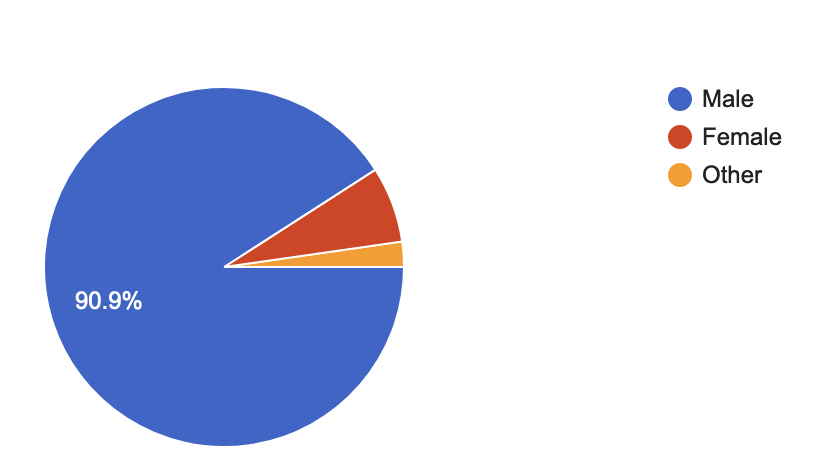
\includegraphics[width=\linewidth]{Images/Survey/demo_1.png}
\caption{Results for - Gender of the participants}
\label{fig:results:demo:1}
\end{figure}

\pagebreak

\subsection*{Your experience in the software engineering field?}

Figure \ref{fig:results:demo:2} presents the distribution of professional experience among the survey participants within the software engineering field. A substantial portion of the respondents, 50\%, possess over ten years of experience, highlighting the survey's capture of seasoned professionals' perspectives. An additional 22.7\% have precisely ten years of experience, further underscoring the experienced nature of the respondent pool. 

This predominance of experienced professionals suggests that the insights derived from this survey are grounded in extensive practical knowledge and awareness of the industry's evolution. However, the representation of those with five years or fewer (27.2\%) introduces a balance, potentially reflecting newer trends and adaptations in software engineering practices. This mixture of veteran and relatively newer engineers can provide a comprehensive overview of the current challenges and effective practices within the field, especially in relation to the adoption of new technologies and methodologies in software engineering.

\begin{figure}[h!]
\centering
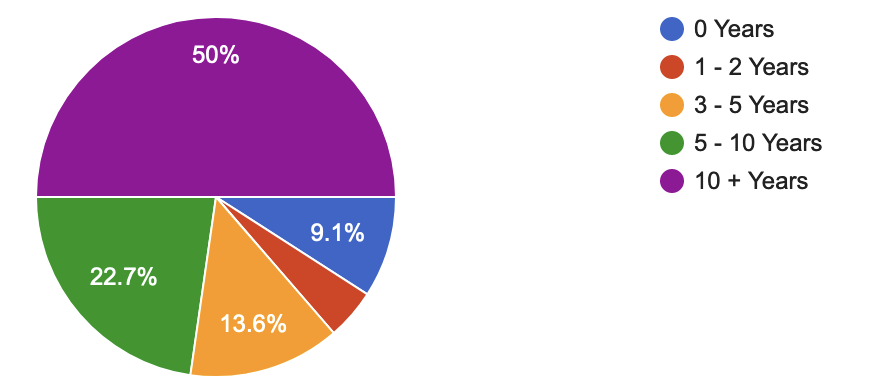
\includegraphics[width=\linewidth]{Images/Survey/demo_2.png}
\caption{Results for - Your experience in the software engineering field?}
\label{fig:results:demo:2}
\end{figure}

\pagebreak

\subsection*{Your level of education or training in software engineering?}
The survey assessed the educational background of the participants within the field of software engineering, revealing a diverse array of educational achievements as shown in Figure \ref{fig:results:demo:3}. The results indicate that 31.8\% of the participants hold a Master's degree or similar, and 29.5\% have a Bachelor's degree, underscoring a highly educated respondent base. Furthermore, a significant 25\% of the participants have gained their skills through self-education or training, reflecting the varied pathways into the software engineering profession.

This educational diversity suggests that the field not only attracts individuals with formal academic training but also those who are self-motivated to learn and adapt outside traditional educational frameworks. This mix of backgrounds may influence team dynamics and the adoption of new technologies, as individuals with different educational experiences might vary in their approaches to learning and integrating new tools. Additionally, the presence of formally trained individuals alongside self-taught professionals can enrich the collaborative environment, potentially leading to more innovative solutions and effective problem-solving within teams.


\begin{figure}[h!]
\centering
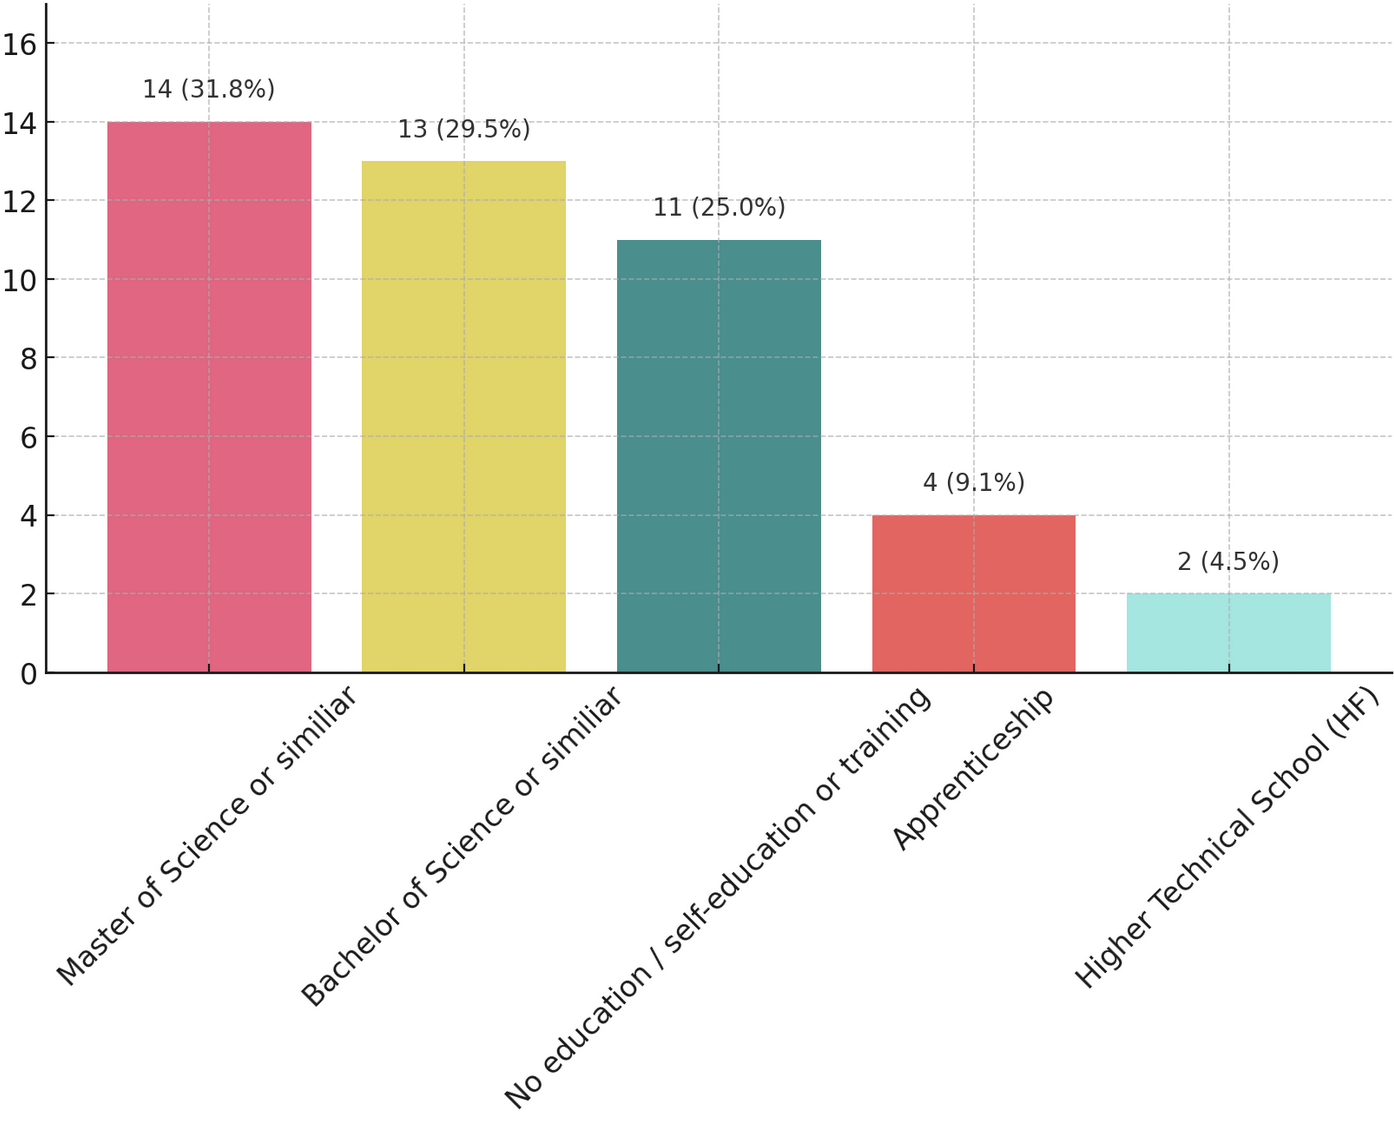
\includegraphics[width=\linewidth]{Images/Survey/demo_3.png}
\caption{Results for - Your level of education or training in software engineering?}
\label{fig:results:demo:3}
\end{figure}

\pagebreak

\subsection*{Your role in a software development team that best suits you.}
The survey assessed the preferred roles of participants within software development teams, showcasing a wide array of career focuses as depicted in Figure \ref{fig:results:demo:4}. The majority of respondents favor technical and design roles, with 29.5\% identifying as Developer/Engineer and 18.2\% as UI/UX Engineers, highlighting a strong inclination towards the foundational and creative aspects of software development.

Moreover, roles such as Project Owner (15.9\%) and QA Engineer (11.4\%) reflect the importance of leadership and quality assurance in software projects, underlining the multifaceted nature of team compositions required to meet today’s complex software development challenges. This diversity in role preference underscores the varied skill sets and perspectives that participants bring to their teams, potentially enriching collaboration and innovation.

The representation of roles across the spectrum from technical to strategic positions suggests that successful software development relies on a balanced integration of various expertises, with each role playing a critical part in the overall project lifecycle and contributing uniquely to the adoption of new technologies and methodologies.


\begin{figure}[h!]
\centering
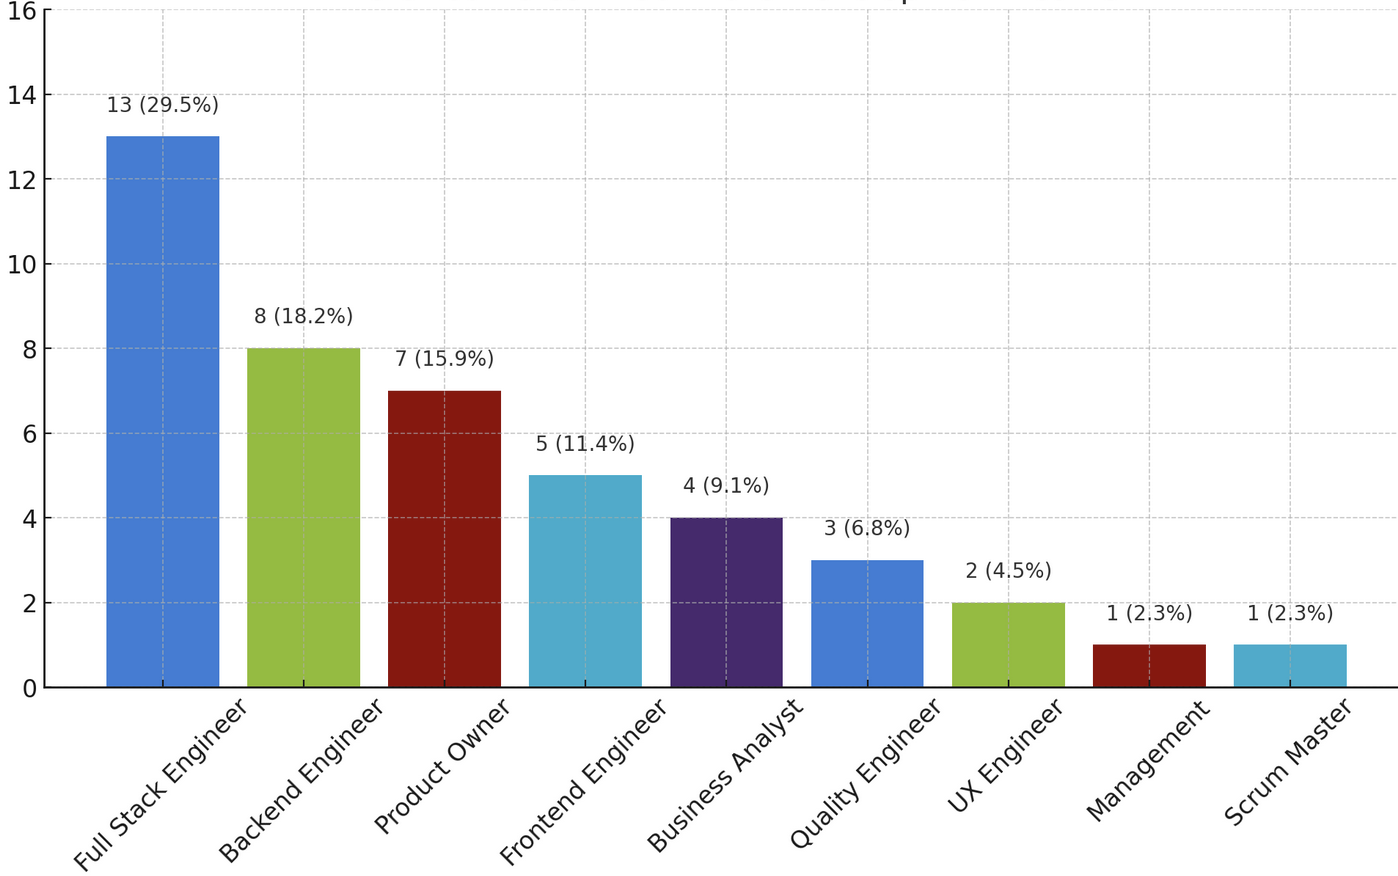
\includegraphics[width=\linewidth]{Images/Survey/demo_4.png}
\caption{Results for - Your role in a software development team that best suits you.}
\label{fig:results:demo:4}
\end{figure}

\pagebreak

\subsection*{Which software development paradigm is normally used in the projects you are involved with?}

The survey queried participants about their preferred software development paradigms, with the results indicating a strong inclination towards Agile and Extreme Programming (XP) methodologies. As illustrated in Figure \ref{fig:results:demo:5}, a significant majority of the participants (84.1\%) employ Agile/XP in their projects, underscoring its prominence in current software engineering practices. The remaining 15.9\% of respondents utilize a mixed approach, incorporating elements from various methodologies to suit specific project needs.

This predominant use of Agile/XP suggests that these methodologies continue to shape the landscape of software development, likely due to their effectiveness in managing complex projects and their adaptability to rapidly changing requirements. The minor yet notable preference for mixed methodologies also highlights a pragmatic approach to software development, where teams adapt and integrate different strategies to optimize outcomes.


\begin{figure}[h!]
\centering
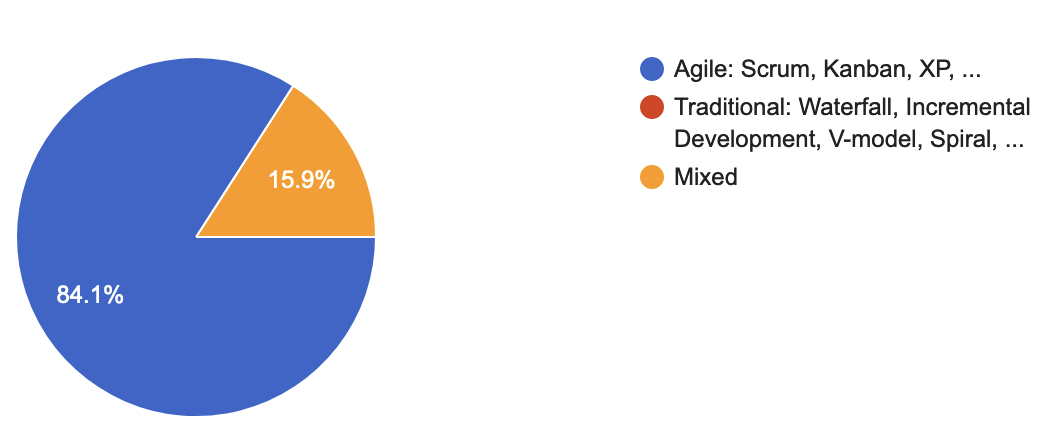
\includegraphics[width=\linewidth]{Images/Survey/demo_5.png}
\caption{Results for - Which software development paradigm is normally used in the projects you are involved with?}
\label{fig:results:demo:5}
\end{figure}

\pagebreak


\section{Role Based Information Highlighting in Documents}

\subsection*{Do you usually get overwhelmed by the amount of information when reading documentations?}
As shown in Figure \ref{fig:results:highlighting:1}, a significant number of respondents experience overwhelm with the volume of information in documentation. The highest frequencies are observed at the upper end of the scale, with 25\% of participants rating their level of overwhelm at 8, and 18.2\% at 7, indicating a notable discomfort. This trend underscores the necessity for improved information structuring and presentation in documentation to aid in better comprehension and usability for software engineering professionals. 


\begin{figure}[h!]
\centering
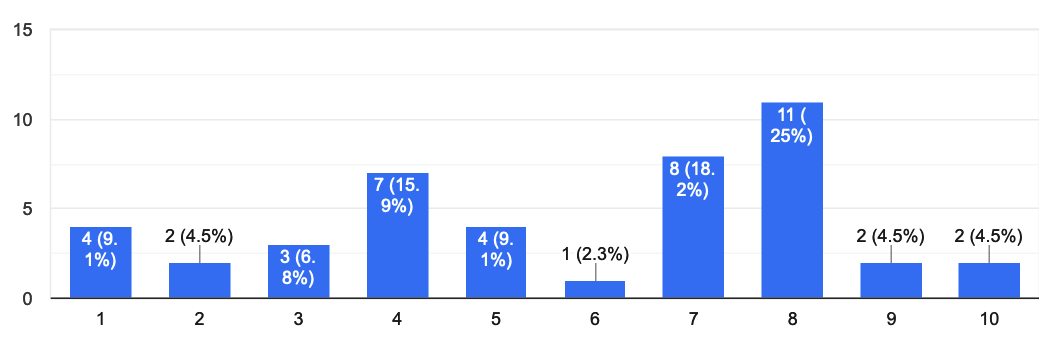
\includegraphics[width=\linewidth]{Images/Survey/documents_1.png}
\caption{Results for - Do you usually get overwhelmed by the amount of information when reading documentations?}
\label{fig:results:highlighting:1}
\end{figure}

\pagebreak

\subsection*{How satisfying would it be to have the information that is most important to you highlighted for you?}
Figure \ref{fig:results:highlighting:2} illustrates a strong positive response to the idea of having key information highlighted in documentation. The majority of the respondents (75\%) expressed high satisfaction (ratings of 8 to 10), highlighting the potential benefit and demand for such features in documentation tools. This response underscores the importance of adaptive and user-centric information presentation, which could significantly enhance readability and efficiency in professional settings.

\begin{figure}[h!]
\centering
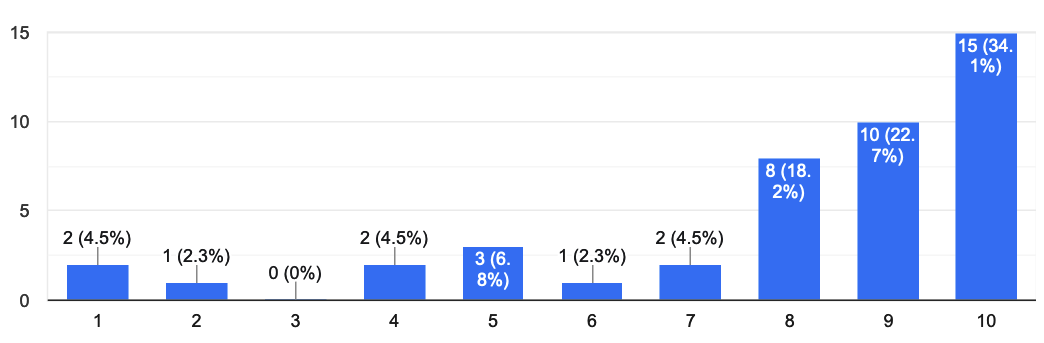
\includegraphics[width=\linewidth]{Images/Survey/documents_2.png}
\caption{Results for - How satisfying would it be to have the information that is most important to you highlighted for you?}
\label{fig:results:highlighting:2}
\end{figure}

\pagebreak


\subsection*{How easy do you think it would be to use \ac{AI} to automate the highlighting of information based on a viewer's role selection?}
Figure \ref{fig:results:highlighting:3} displays a diverse range of opinions regarding the ease of using \ac{AI} for automated information highlighting. The data shows a notable spread across the scale with a concentration in the moderate-to-high feasibility range (ratings of 6 to 7), indicating a cautious optimism. This suggests a recognition of \ac{AI}'s potential, paired with an awareness of the practical and technical challenges that might be encountered. The mixed responses underscore the need for ongoing research and development to enhance \ac{AI}'s capabilities and ease of integration into existing workflows, especially in complex fields such as software engineering.

\begin{figure}[h!]
\centering
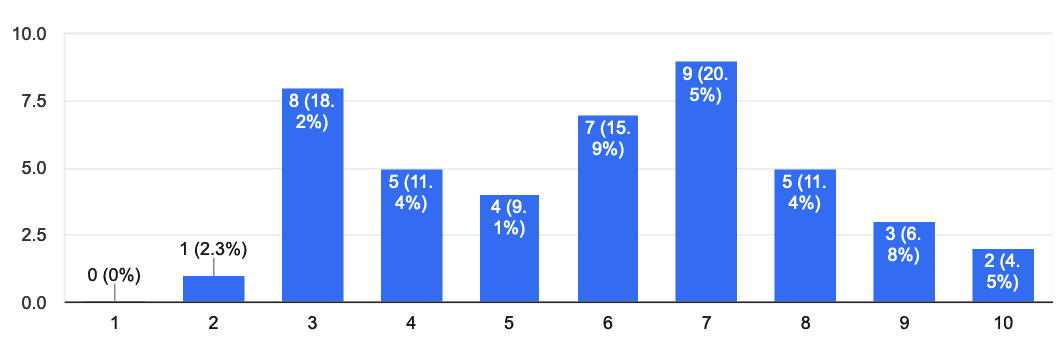
\includegraphics[width=\linewidth]{Images/Survey/documents_3.png}
\caption{Results for - How easy do you think it would be to use \ac{AI} to automate the highlighting of information based on a viewer's role selection?}
\label{fig:results:highlighting:3}
\end{figure}

\pagebreak

\subsection*{How much better do you think this approach of highlighting just the right information is than having separate pages for different roles?}
Figure \ref{fig:results:highlighting:4} illustrates a positive reception towards the highlighting approach over having separate pages for different roles. A majority of respondents (59.1\%) rated the benefit of this approach as high (7 to 10 on the scale), underscoring the perceived efficiency and effectiveness of integrating information in a single document with role-specific highlights. This preference highlights the potential for tools that can intelligently adapt content presentation to user needs, enhancing usability and accessibility in professional settings. However, a significant proportion of participants showed some reservations, indicating a need for further exploration into the implementation challenges and accuracy of such \ac{AI}-driven solutions.
\begin{figure}[h!]
\centering
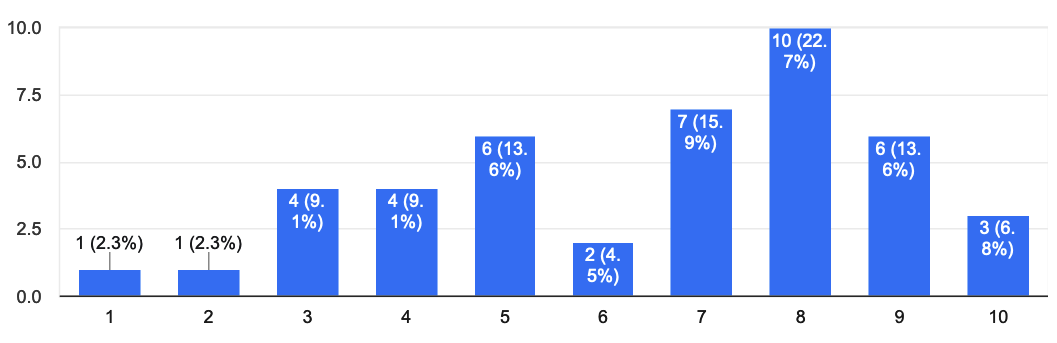
\includegraphics[width=\linewidth]{Images/Survey/documents_4.png}
\caption{Results for - How easy do you think it would be to use \ac{AI} to automate the highlighting of information based on a viewer's role selection?}
\label{fig:results:highlighting:4}
\end{figure}

\pagebreak

\subsection*{In your personal experience, do you see people using more text or screenshots to document information?}
Figure \ref{fig:results:highlighting:5} depicts a varied spectrum of preferences between text and screenshots in documentation practices. A substantial number of participants lean towards a balanced or slightly higher use of screenshots (scale points 4 to 8), indicating a preference for visual documentation elements in certain contexts. This suggests that while traditional text-based documentation remains foundational, the integration of visual elements like screenshots is becoming increasingly prevalent, possibly due to their ability to convey complex information more effectively and engagingly. This trend underscores the need for tools and practices that seamlessly integrate both textual and visual information to accommodate diverse documentation needs and preferences.

\begin{figure}[h!]
\centering
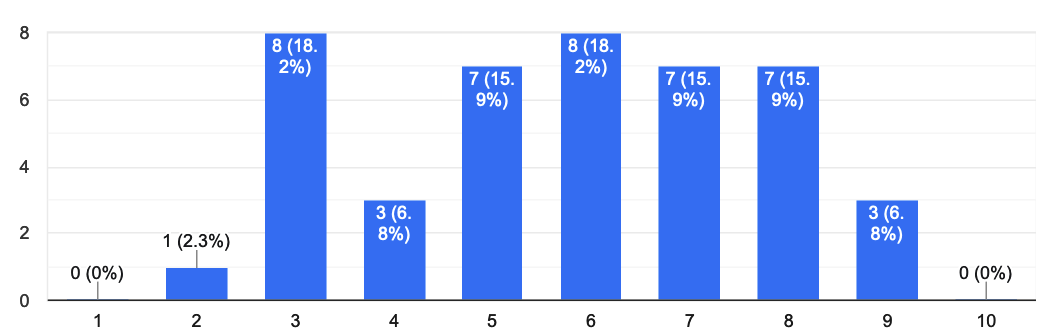
\includegraphics[width=\linewidth]{Images/Survey/documents_5.png}
\caption{Results for - In your personal experience, do you see people using more text or screenshots to document information?}
\label{fig:results:highlighting:5}
\end{figure}

\pagebreak

\section{Decision Logs Within a Mirrored Approach}

\subsection*{How important do you think it is to have a record of decisions and an up-to-date record of decisions?}
Figure \ref{fig:results:decisions:1} illustrates a strong consensus among participants on the importance of maintaining a thorough and current record of decisions. A significant majority (70.5\%) rated this necessity highly (8 to 10 on the scale), highlighting the critical role that decision logs play in ensuring transparency, continuity, and accountability in organizational processes. This strong endorsement underlines the need for robust systems and practices that can reliably document and update decision records, serving as a foundational aspect of effective project management and operational efficiency.

\begin{figure}[h!]
\centering
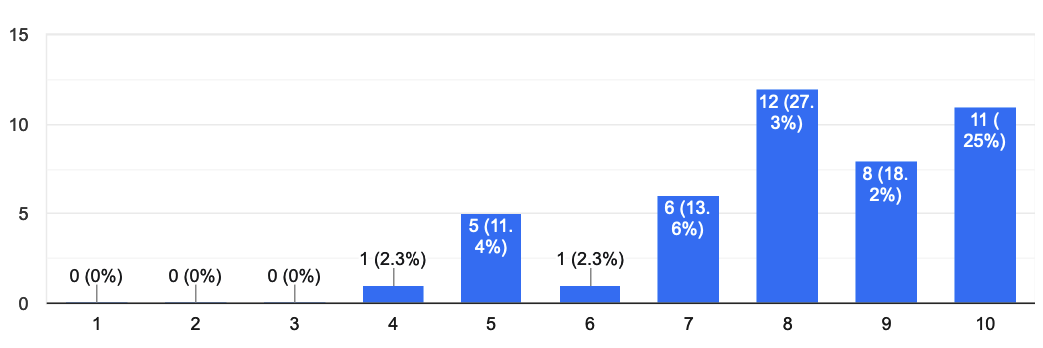
\includegraphics[width=\linewidth]{Images/Survey/decisions_1.png}
\caption{Results for - How important do you think it is to have a record of decisions and an up-to-date record of decisions?}
\label{fig:results:decisions:1}
\end{figure}

\pagebreak

\subsection*{Did the decision logs you've seen so far contain the most up-to-date information, were they properly formatted and did they make sense?}
Figure \ref{fig:results:decisions:2} presents a mixed response to the quality of decision logs encountered by participants. While a small segment of respondents (29.5\%) expressed relatively high satisfaction (ratings 7 to 10), the majority (65.9\%) rated their experience with decision logs as average to poor (ratings 1 to 6). This underscores a critical need for improvements in how decision logs are maintained and formatted. Ensuring that decision logs are up-to-date, clear, and logically structured is paramount to their utility in guiding and documenting project decisions effectively.

\begin{figure}[h!]
\centering
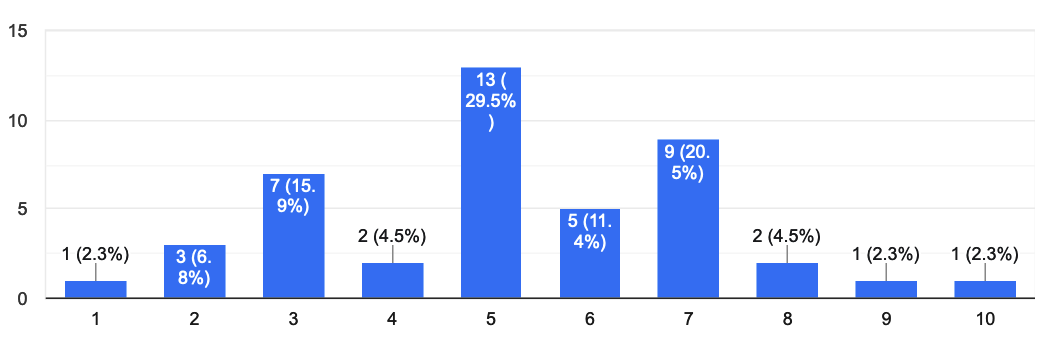
\includegraphics[width=\linewidth]{Images/Survey/decisions_2.png}
\caption{Results for - Did the decision logs you've seen so far contain the most up-to-date information, were they properly formatted and did they make sense?}
\label{fig:results:decisions:2}
\end{figure}

\pagebreak

\subsection*{How do you think the decision logs would benefit from being part of the relevant code base, rather than a separate document, in terms of being up to date?}
Figure \ref{fig:results:decisions:3} reveals a strong preference among participants for integrating decision logs directly within the code base. The majority of respondents (68\%) perceive high benefits (ratings 7 to 10) from such integration, emphasizing its potential to keep decision records more current and closely tied to the actual code changes they pertain to. This approach could enhance the accuracy and timeliness of decision logs, making them more dynamic and immediately relevant. However, a considerable minority expressed reservations, highlighting the need for careful consideration of implementation strategies to address potential barriers and optimize usability for all stakeholders.

\begin{figure}[h!]
\centering
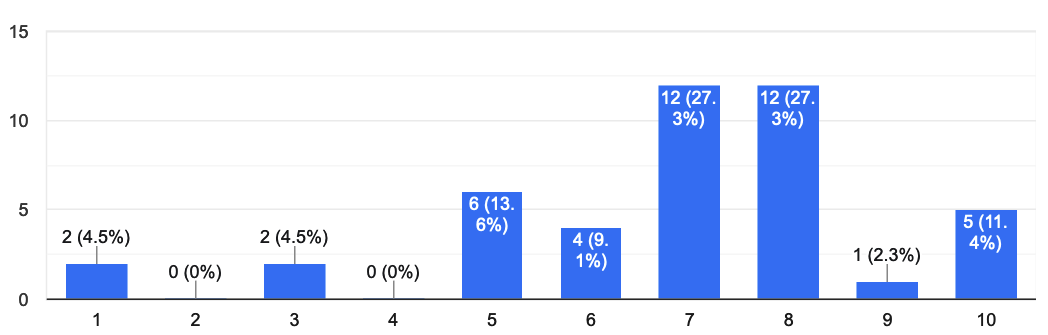
\includegraphics[width=\linewidth]{Images/Survey/decisions_3.png}
\caption{Results for - How do you think the decision logs would benefit from being part of the relevant code base, rather than a separate document, in terms of being up to date?}
\label{fig:results:decisions:3}
\end{figure}

\pagebreak

\subsection*{How important do you think it is, if the decision logs are in the associated codebase, to still keep them in a document accessible to "non-developers"?}
Figure \ref{fig:results:decisions:4} demonstrates a significant valuation of making decision logs accessible to non-developers, with over half of the respondents (52.3\%) rating this importance highly (8 to 10). This underlines the perceived need for transparency and inclusivity in project documentation, facilitating broader understanding and engagement across all stakeholders. However, nearly half of the participants expressed less concern, highlighting diverse views on the operational and security challenges of broadly accessible decision logs. This dichotomy suggests a need for balanced solutions that cater to the needs of diverse project teams while ensuring that decision logs remain comprehensible and secure.

\begin{figure}[h!]
\centering
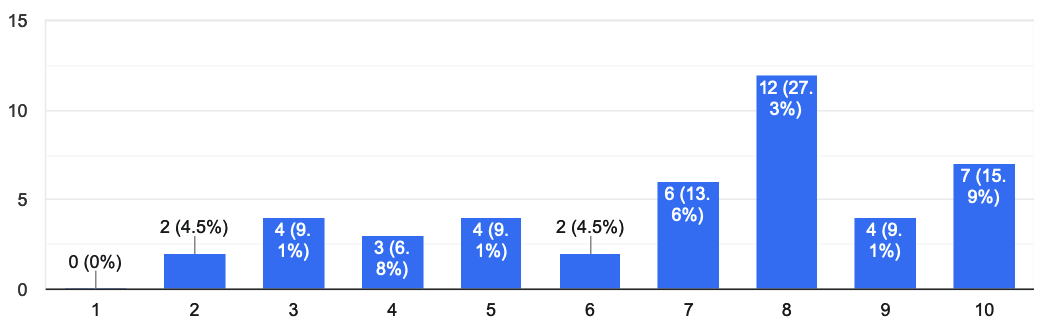
\includegraphics[width=\linewidth]{Images/Survey/decisions_4.png}
\caption{Results for - How important do you think it is, if the decision logs are in the associated codebase, to still keep them in a document accessible to "non-developers"?}
\label{fig:results:decisions:4}
\end{figure}

\pagebreak


\subsection*{How easy do you think it would be to use tools to automate the mirroring of decisions into a separate document accessible to everyone?}
Figure \ref{fig:results:decisions:5} indicates a wide range of opinions regarding the ease of using tools to automate the mirroring of decision logs. While a moderate number of respondents (52.3\% with ratings 4 to 7) believe that it is reasonably feasible, a significant portion (29.5\% with ratings 1 to 3) express reservations, suggesting perceived complexities or usability issues with existing tools. On the other hand, a smaller segment (18.2\% with ratings 8 to 10) shows strong confidence in the current capabilities of such tools. This spread of responses highlights the need for further research into tool development, focusing on enhancing user-friendliness and integration capabilities to support effective decision log management across diverse teams.

\begin{figure}[h!]
\centering
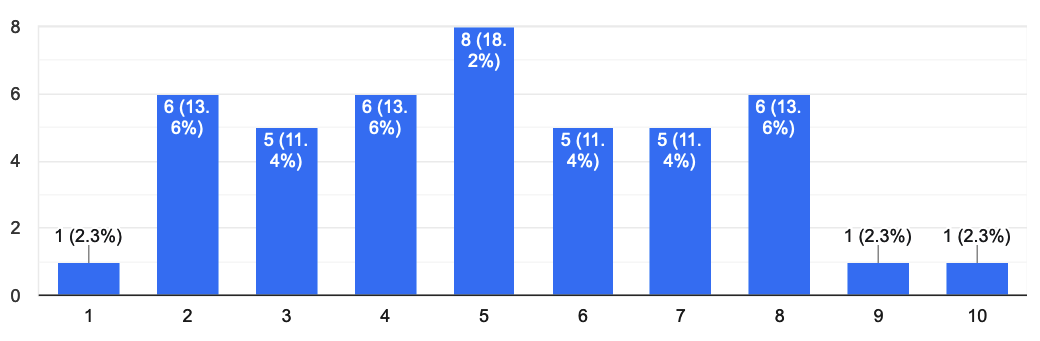
\includegraphics[width=\linewidth]{Images/Survey/decisions_5.png}
\caption{Results for - How easy do you think it would be to use tools to automate the mirroring of decisions into a separate document accessible to everyone?}
\label{fig:results:decisions:5}
\end{figure}

\pagebreak


\section{Infrastructure as Code}

\subsection*{In your current software project, how much do you know about how deployments and architectures work?}
Figure \ref{fig:results:iac:1} reflects varied levels of understanding among participants regarding the deployments and architectures in their software projects. Nearly half of the respondents (47.7\%) report high knowledge (ratings of 8 to 10), showcasing a strong command over technical aspects of their projects. This level of proficiency is crucial for effective project management and could potentially influence the adoption and success of \ac{IaC} practices. Meanwhile, the substantial number of moderate responses (38.6\%) signals areas where targeted educational initiatives could further enhance team capabilities and project outcomes.

\begin{figure}[h!]
\centering
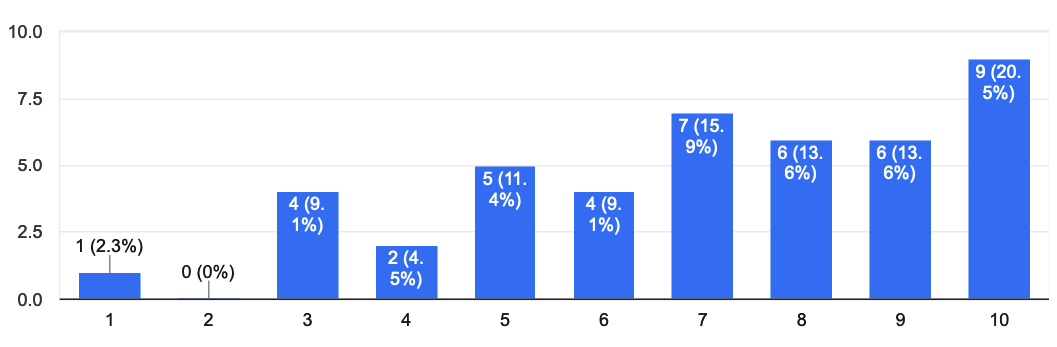
\includegraphics[width=\linewidth]{Images/Survey/iac_1.png}
\caption{In your current software project, how much do you know about how deployments and architectures work?}
\label{fig:results:iac:1}
\end{figure}

\pagebreak


\subsection*{How familiar are you with the concept of IaC and its benefits?}
Figure \ref{fig:results:iac:2} illustrates a wide spectrum of familiarity with the concept of \ac{IaC} among the survey participants. Notably, a significant portion of the respondents (38.6\%) possess limited knowledge of \ac{IaC}, as indicated by the low ratings (1 to 4). This suggests a potential barrier to the full adoption and optimization of \ac{IaC} practices within their projects. On the other hand, nearly 30\% of the participants demonstrate a high understanding (ratings of 8 to 10), which could indicate a readiness to implement or enhance \ac{IaC} solutions effectively. The results underscore the need for targeted educational programs that could bridge the knowledge gap and facilitate a deeper understanding and utilization of \ac{IaC} benefits across software teams.
\begin{figure}[h!]
\centering
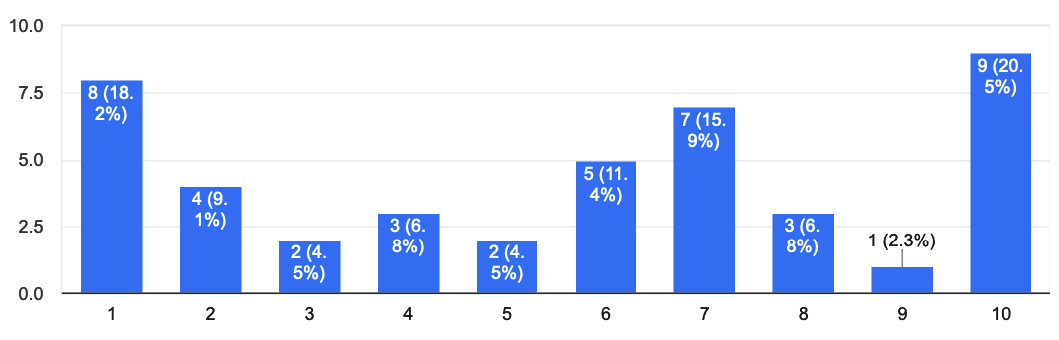
\includegraphics[width=\linewidth]{Images/Survey/iac_2.png}
\caption{How familiar are you with the concept of IaC and its benefits?}
\label{fig:results:iac:2}
\end{figure}

\pagebreak

\subsection*{To what extent do you agree that IaC helps in fostering a sense of shared responsibility among development team members?}

Figure \ref{fig:results:iac:3} indicates a predominantly positive reception to the role of \ac{IaC} in fostering shared responsibility among team members, with over half of the respondents (52.3\%) expressing high agreement (ratings 7 to 10). This response suggests that \ac{IaC} is viewed not only as a technical tool but also as a facilitator of collaborative and accountable practices within development teams. However, a significant proportion of participants (36.4\%) provided moderate responses, highlighting potential variability in experiences or perceptions of \ac{IaC}'s effectiveness in this regard. This mixed response underscores the need for further investigation into how \ac{IaC} practices are implemented and perceived across different team environments and project contexts.

\begin{figure}[h!]
\centering
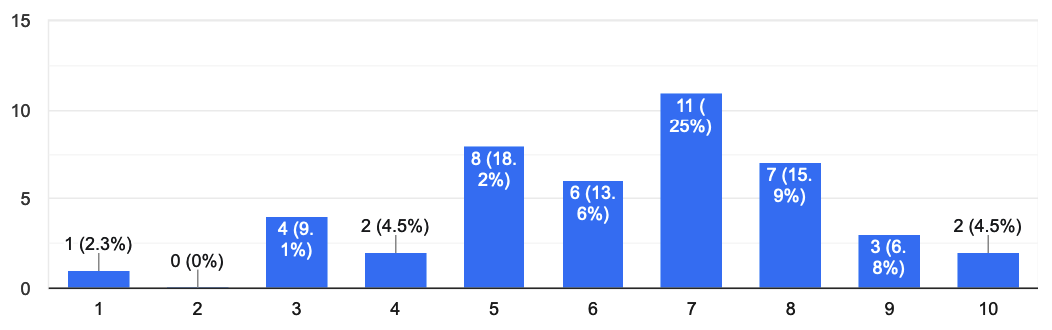
\includegraphics[width=\linewidth]{Images/Survey/iac_3.png}
\caption{To what extent do you agree that IaC helps in fostering a sense of shared responsibility among development team members?}
\label{fig:results:iac:3}
\end{figure}

\pagebreak

\subsection*{What are the biggest challenges or limitations you have faced when implementing IaC in your projects?}
The survey elicited detailed feedback on the challenges faced by software engineering professionals when implementing \ac{IaC}. As depicted in the responses, a significant range of obstacles impacts the adoption and effective use of \ac{IaC} technologies.

\textbf{Complexity and Knowledge Gaps:} Respondents highlighted the inherent complexity involved in managing and understanding intricate infrastructure configurations, particularly in larger-scale projects. This complexity is exacerbated by gaps in necessary skills, with several participants noting the steep learning curve associated with mastering domain-specific configuration languages and tools like Terraform.

\textbf{Migration and Adaptation:} Legacy systems pose substantial challenges, with their migration to \ac{IaC} described as particularly difficult. Issues in modifying existing, often poorly structured configuration files further complicate transitions to \ac{IaC} practices.

\textbf{Team Dynamics and Expertise Concentration:} A recurring theme in the responses was the concentration of \ac{IaC} knowledge within small subsets of teams, leading to knowledge silos and dependency on few individuals. This situation poses risks in knowledge continuity and creates barriers for broader team involvement.

\textbf{Security and Operational Risks:} Security emerged as a critical concern, with respondents expressing worries about accidentally exposing resources due to misconfigurations. The operational challenges of testing and rapidly adapting \ac{IaC} configurations in dynamic environments were also noted as significant hurdles.

These insights underline the need for comprehensive strategies to enhance training, improve documentation and knowledge sharing, and foster more inclusive team involvement in \ac{IaC} practices to mitigate these challenges effectively.


\section{Summary}

\subsection*{In your opinion, what combination of techniques would be the most effective?}

This question sought to identify which combinations of development techniques are perceived as the most effective by participants. The results highlight a clear preference for integrating specific approaches to enhance the overall software development process.

\begin{itemize}
    \item \textbf{Role-Based Information Highlighting + Decision Logs Mirroring:} This combination received the most endorsements, with 12 participants highlighting its effectiveness. The integration of role-based information highlighting with mirrored decision logs likely offers significant improvements in ensuring that all team members have access to the necessary information in a format that supports effective decision-making and accountability.

    \item \textbf{Decision Logs Mirroring + Infrastructure as Code:} With 9 votes, this pairing underscores the value of maintaining transparent and traceable changes within automated infrastructure setups, suggesting that decision logs mirroring complements the precision and automated nature of IaC.

    \item \textbf{Infrastructure as Code + Role-Based Information Highlighting:} Although it received fewer votes (7 participants), the combination of tailored information delivery with automated infrastructure management is recognized as beneficial, particularly for managing complex environments efficiently and accurately.
\end{itemize}


%---------------------------------------------------------------------------------------- 


%----------------------------------------------------------------------------------------
% THESIS CONTENT - APPENDICES
%----------------------------------------------------------------------------------------
\appendix % Cue to tell LaTeX that the following "chapters" are Appendices

% Include the appendices of the thesis as separate files from the Appendices folder
% Uncomment the lines as you write the Appendices
% !TEX root = ../main.tex

%----------------------------------------------------------------------------------------
% APPENDIX A
%----------------------------------------------------------------------------------------

\chapter{Frequently Asked Questions} % Main appendix title

\label{AppendixA} % For referencing this appendix elsewhere, use \ref{AppendixA}

\section{How do I change the colors of links?}

The color of links can be changed to your liking using:

{\small\verb!\hypersetup{urlcolor=red}!}, or

{\small\verb!\hypersetup{citecolor=green}!}, or

{\small\verb!\hypersetup{allcolor=blue}!}.

\noindent If you want to completely hide the links, you can use:

{\small\verb!\hypersetup{allcolors=.}!}, or even better: 

{\small\verb!\hypersetup{hidelinks}!}.

\noindent If you want to have obvious links in the PDF but not the printed text, use:

{\small\verb!\hypersetup{colorlinks=false}!}

\section{How can I add a Figure in the Appendix?}

You can refer to a figure in the Appendix (like \ref{fig:appendix-figure}) and it will show up as expected.

\begin{figure}

\includegraphics[width=0.25\textwidth]{../Figures/Bart_Simpson.png}
\centering
\caption[A random appendix figure]{Bart Simpson. (2023, May 17). In Wikipedia. \url{https://en.wikipedia.org/wiki/Bart_Simpson}}
\label{fig:appendix-figure}
\end{figure}

% from https://www.zhaw.ch/en/lsfm/study/studiweb/master-ls/masters-thesis/
%\include{Appendices/AppendixB}
%\include{Appendices/AppendixC}
% Appendix: Declaration of Originality

\chapter{Declaration of Originality} % Main appendix title

\label{DeclarationOfOriginalityZHAW} % For referencing this appendix elsewhere, use \ref{AppendixA}


\includepdf[pages=-]{Appendices/plagiatserklaerung-master-eng.pdf}
 


%----------------------------------------------------------------------------------------
% BIBLIOGRAPHY
%----------------------------------------------------------------------------------------
\printbibliography[heading=bibintoc]

%----------------------------------------------------------------------------------------

\end{document}  
